\documentclass[letterpaper]{article}
\usepackage[square,sort,comma,numbers]{natbib}
\usepackage{array}
%====================================================================%
../../../../tex/scufftex.tex
\graphicspath{{figures/}}
\renewcommand{\wt}{\widetilde}

%------------------------------------------------------------
%------------------------------------------------------------
%- Special commands for this document -----------------------
%------------------------------------------------------------
%------------------------------------------------------------

%------------------------------------------------------------
%------------------------------------------------------------
%- Document header  -----------------------------------------
%------------------------------------------------------------
%------------------------------------------------------------
\title {Implicit handling of multilayered dielectric substrates 
        in {\sc scuff-static}
       }
\author {Homer Reid}
\date {April 3, 2017}

%------------------------------------------------------------
%------------------------------------------------------------
%- Start of actual document
%------------------------------------------------------------
%------------------------------------------------------------

\begin{document}
\pagestyle{myheadings}
\markright{Homer Reid: Electrostatic GF above PCB} 
\maketitle

\tableofcontents

%====================================================================%
%====================================================================%
%====================================================================%
\newpage
%####################################################################%
\begin{figure}
\begin{center}
\resizebox{\textwidth}{!}{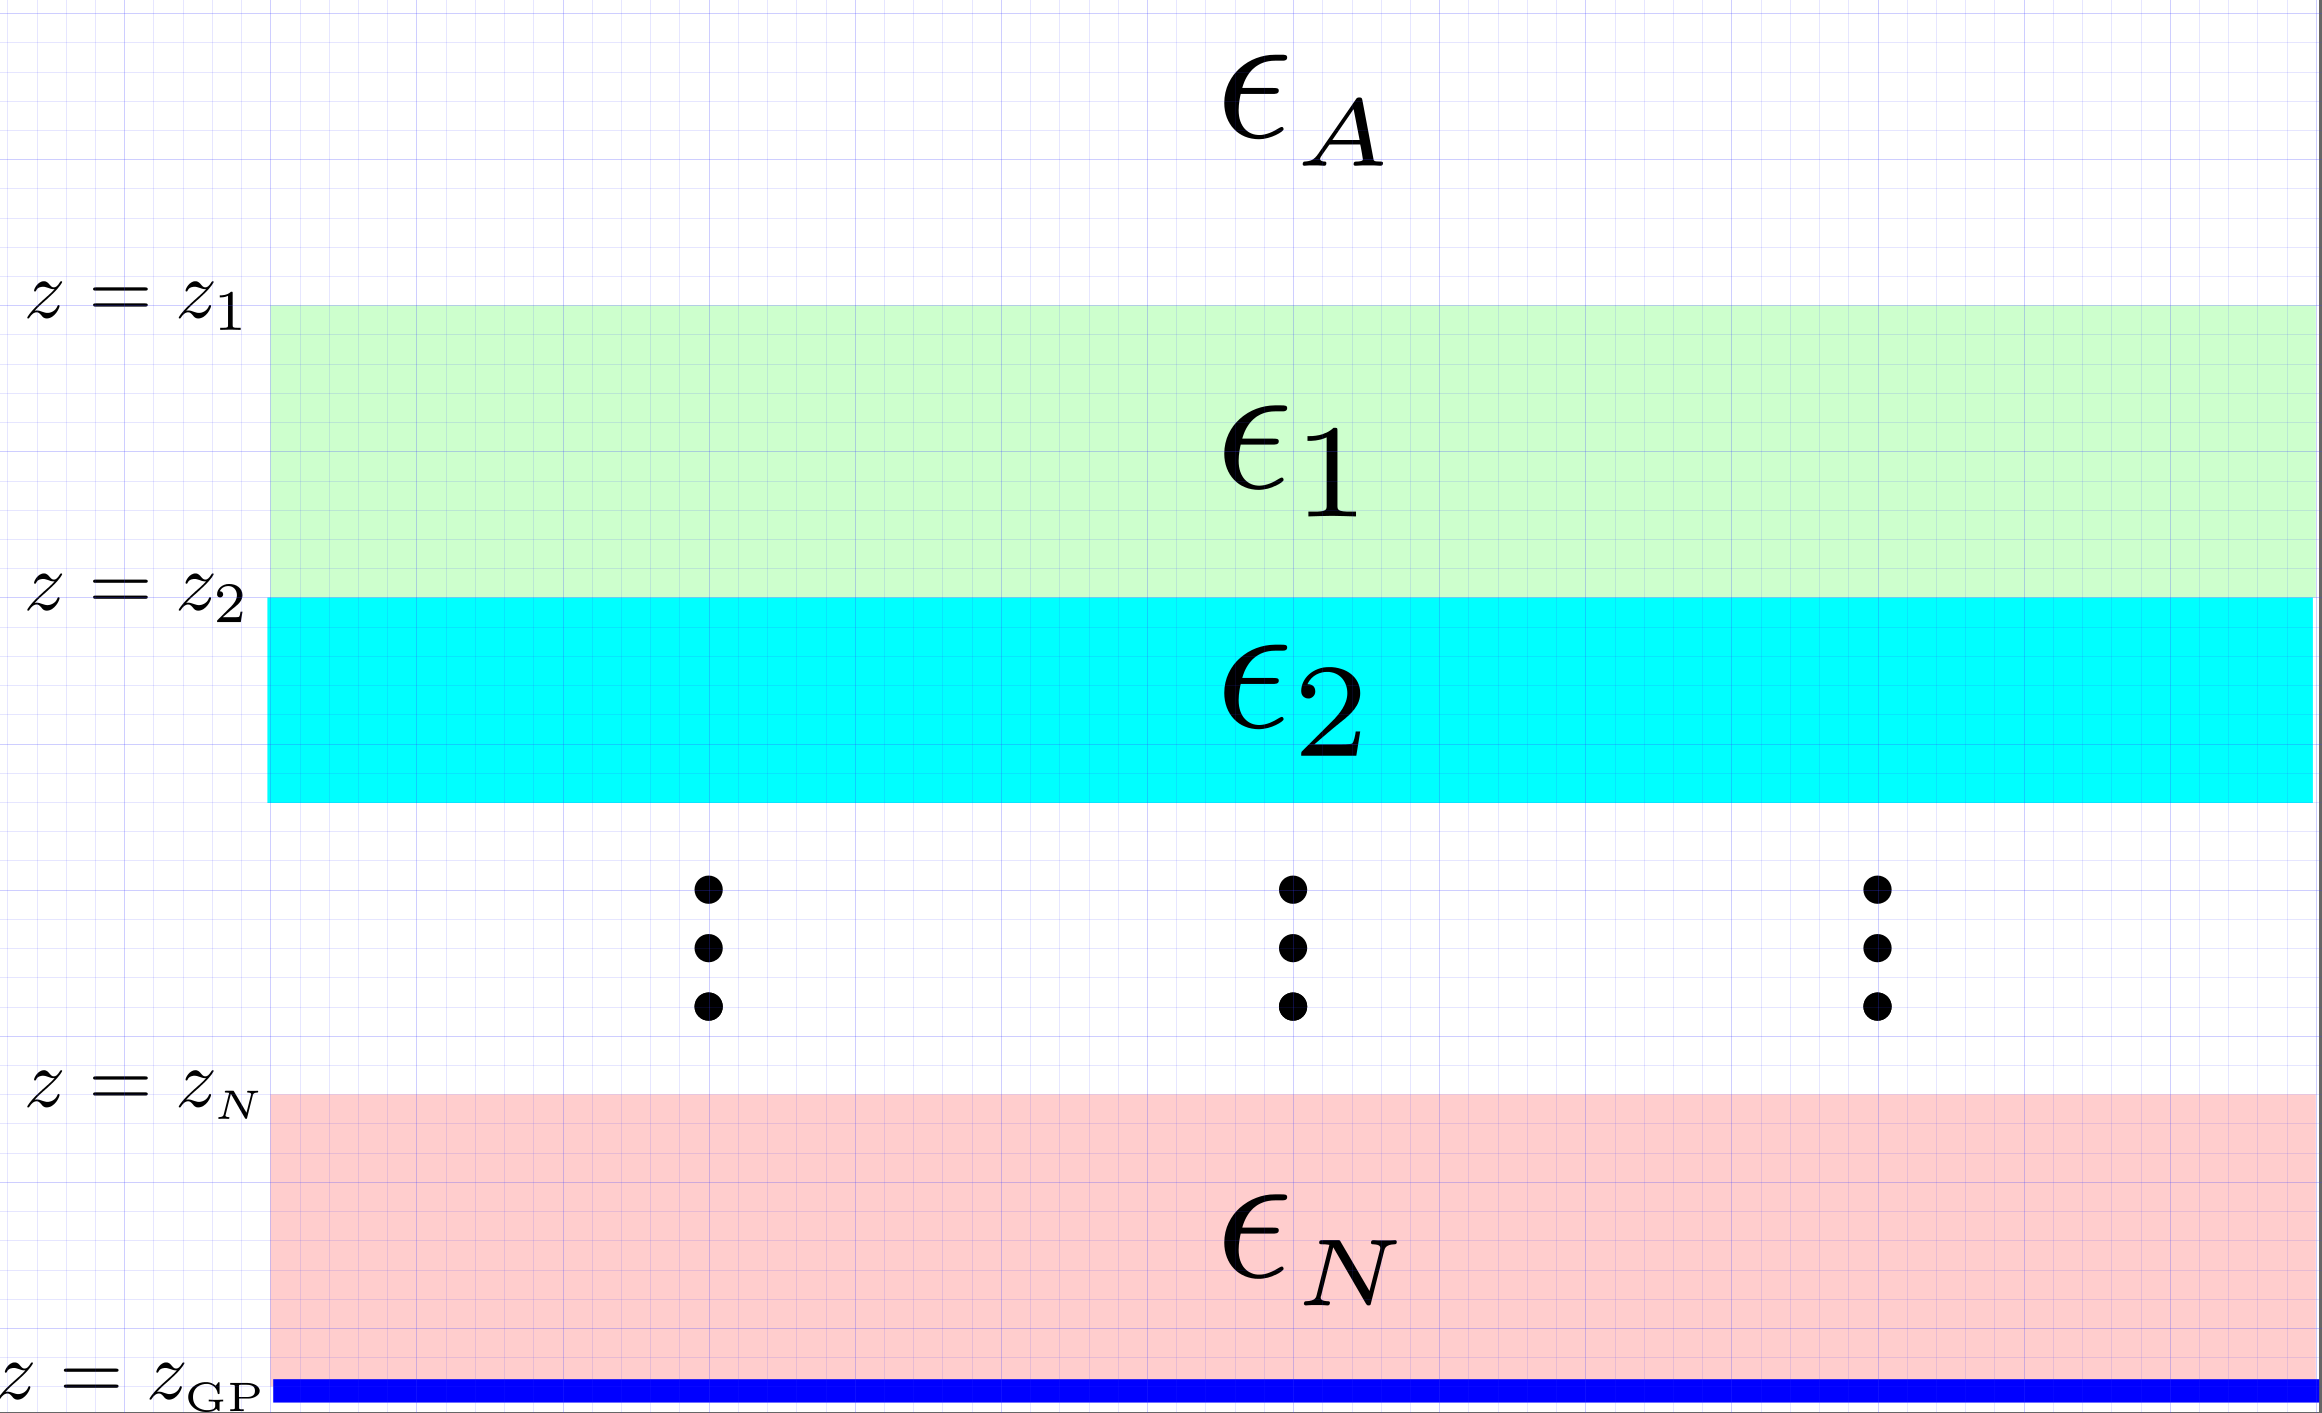
\includegraphics{DielectricSubstrateCartoon.pdf}}
\caption{Geometry of the layered dielectric substrate. The $n$th layer
has relative DC permittivity $\epsilon_n$, and its upper surface
lies at $z=z_n$. The ground plane, if present, lies
at $z=z\subt{GP}.$ The upper medium, if not vacuum, has permittivity
$\epsilon\subt{A}.$}
\label{SubstrateGeometryFigure}
\end{center}
\end{figure}
%####################################################################%
\section{Overview}

In this memo I describe an extension to the {\sc scuff-em}
electrostatics module to allow implicit treatment of
layered substrates consisting of multiple dielectric layers,
of arbitrary thicknesses and permittivities, with an optional
perfectly conducting ground plane (Figure 1).\footnote{Note 
that, if there is no ground plane, then the bottommost 
layer in Figure \ref{SubstrateGeometryFigure}
(layer $N$) is assumed
to be infinitely thick (it has no lower surface). Thus, a physical 
substrate consisting of $M$ finite-thickness dielectric layers with 
no ground plane is treated here as a stack of $N=M+1$ layers in which
the bottommost layer is vacuum, i.e. $\epsilon\subt{$N$}=1.$}

Proceeding in reverse order from theory to practice, the 
structure of this memo is as follows:

\begin{itemize}
\item 
In Section \ref{ImplementationSection} I discuss the usage
of this new feature in {\sc scuff-em} electrostatics calculations.

\item 
In Section \ref{TheorySection} I discuss the physics and
mathematics of the underlying method and some technical details
regarding its implementation in {\sc scuff-em}.
\end{itemize}

%====================================================================%
%====================================================================%
%====================================================================%
\newpage
\section{Practice: Running {\sc scuff-em} calculations
         with implicit substrates}
\label{ImplementationSection}

%=================================================
%=================================================
%=================================================
\subsection{Substrate definition file}

Referring to Figure \ref{SubstrateGeometryFigure},
a substrate geometry is specified by
\begin{itemize}
 \item the $z$-coordinate of the upper surface of each dielectric layer
 \item the permittivity of each layer
 \item the $z$-coordinate of the optional ground plane.
\end{itemize}

This data is specified to {\sc scuff-em} in the
form of a simple text file (conventionally given file
extension \texttt{.substrate}) consisting of one line for each
dielelectric layer plus an optional line specifying the ground 
plane, of the form

\medskip

%====================================================================%
\begin{verbcode}
z1  Material1
z2  Material2
...
zN  MaterialN
zGP GROUNDPLANE
\end{verbcode}
%====================================================================%

\medskip

where e.g.
%====================================================================%
\begin{itemize}
 \item \texttt{z1} is the $z$-coordinate of the upper surface of
       layer 1
 \item \texttt{Material1} is a {\sc scuff-em} material designation
       describing the material of layer 1
 \item The optional 
       final line, which invokes the fixed keyword \texttt{GROUNDPLANE},
       specifies that a perfectly-conducting ground plane lives at 
       coordinate $z=\texttt{zGP}$.
\end{itemize}
If the medium above the uppermost dielectric layer is not vacuum,
its permittivity may be specified by including a line of the form
$\texttt{MEDIUM UpperMaterial}.$
%====================================================================%

Note that, because of the scale invariance of electrostatics,
there is no intrinsic length unit here; instead, numerical values
specified for $z_n$ refer to the same length units---be they
microns, millimeters, or what have you--- used in mesh files 
and \texttt{--EPFile}s.

Here are some examples of \texttt{.substrate} files:

\begin{itemize}

\item An infinite-thickness dielectric slab with $\epsilon_r=4$ filling
the lower half-space:

\medskip
%====================================================================%
\begin{verbcode}
0 CONST_EPS_4
\end{verbcode}
%====================================================================%
\medskip

\item A finite-thickness dielectric slab with $\epsilon_r=4$
and thickness 1 whose upper surface is the $xy$ plane:

%====================================================================%
\medskip
\begin{verbcode}
 0 CONST_EPS_4
-1 VACUUM
\end{verbcode}
%====================================================================%

\item The same finite-thickness slab as before, but now 
lying atop a ground plane:

%====================================================================%
\medskip
\begin{verbcode}
 0 CONST_EPS_4
-1 GROUNDPLANE
\end{verbcode}
\medskip
%====================================================================%

\item A unit-thickness layer of $\epsilon_r=4$ atop an infinite-thickness
slab of silicon:

%====================================================================%
\medskip
\begin{verbcode}
 0 CONST_EPS_4
-1 SILICON
\end{verbcode}

\item A unit-thickness layer of $\epsilon_r=4$ atop a thickness-2 layer 
of silicon:

%====================================================================%
\medskip
\begin{verbcode}
 0 CONST_EPS_4
-1 SILICON
-3 VACUUM
\end{verbcode}

\item Same as previous item, but now with a ground plane beneath
the silicon layer:

%====================================================================%
\medskip
\begin{verbcode}
 0 CONST_EPS_4
-1 SILICON
-3 GROUNDPLANE
\end{verbcode}
\medskip
%====================================================================%
\end{itemize}

%=================================================
%=================================================
%=================================================
\subsection{Including implicit substrates in {\sc scuff-em} electrostatics
            calculations}

To run {\sc scuff-em} electrostatics calculations with an implicit 
substrate described by a file \texttt{MySubstrate.substrate},
there are two ways to proceed.

\begin{itemize}
 \item You can include the line

       \begin{verbcode}
         SUBSTRATE MySubstrate.substrate
       \end{verbcode}

       to the \texttt{.scuffgeo} file defining the meshed geometry.
       Then the substrate will be present for all calculations---including
       both API calculations and command-line calculations---involving 
       that geometry file.
 \item For command-line calculations, you can add the option

       \begin{verbcode}
       --SubstrateFile MySubstrate.substrate
       \end{verbcode}

       to the {\sc scuff-static} command line. 
       The substrate file specified in this way will override
       any \texttt{SUBSTRATE} specification that may be present
       in the \texttt{.scuffgeo} file.
\end{itemize}

%====================================================================%
%====================================================================%
%====================================================================%
\newpage
\section{Theory: How it works}
\label{TheorySection}
This discussion consists of two parts:
\begin{itemize}
 \item
 I first derive a mathematical expression for the electrostatic
 Green's function in the presence of the multilayered dielectric
 substrate---that is, the function $G(\vb x\subt{D},\vb x\subt{S})$
 giving the electrostatic potential at $\vb x\subt{D}$ due to a
 unit-strength point source at $\vb x\subt{S}$ in the 
 presence of the substrate (Figure \ref{SigmaLayersFigure}).
 (The subscripts ``D'' and ``S'' stand for ``destination'' and ``source.'')

 \item
 Then I discuss how the discretized surface-integral-equation
 system assembled by {\sc scuff-em} is modified to accommodate
 this modified Green's function.
\end{itemize}

%=================================================
%=================================================
%=================================================
\subsection{Electrostatic Green's function in the presence of
            dielectric substrate}
%####################################################################%
\begin{figure}
\begin{center}
\resizebox{\textwidth}{!}{\includegraphics{DielectricSubstrateSigmaLayers.pdf}}
\caption{In the surface-integral-equation picture of the geometry of Figure
         \ref{SubstrateGeometryFigure}, the effect of the dielectric substrate
         is represented by a collection of surface-charge layers
         $\{\sigma_{n}(\vbrho)\}$, where $\sigma_n$ lives at the 
         upper surface of dielectric layer $n$, i.e. at $z=z_n$.}
\label{SigmaLayersFigure}
\end{center}
\end{figure}
%####################################################################%

\subsubsection{Basic strategy}

In keeping with the spirit of the surface-integral-equation method, I
will
proceed by determining the effective surface-charge densities
induced at each dielectric interface by the point source
(Figure \ref{SigmaLayersFigure}). For an $N$-layer substrate
there are $N$ such layers, with the surface-charge density at
the interface between layers $n-1$ and $n$ denoted by $\sigma_n(\vbrho)$.
Note that I do not include a
surface-charge layer for the ground plane, whose effect I capture
implicitly via the method of images. 

\subsubsection{Expressing $G$ in terms of $\sigma$}

I write the full Green's function $G(\vb x\subt{D}, \vb x\subt{S})$---the 
potential at $\vb x\subt{D}=(\vbrho\subt{D},z\subt{D})$ 
due to a unit-strength\footnote{I assume that charge is measured
in units of $\frac{1}{\epsilon_0}$ (the inverse vacuum permittivity),
so that there is no factor of $\epsilon_0$ in the denominators
of expressions like (\ref{GTotal}).} point charge
at $\vb x\subt{S}=(\vbrho\subt{S},z\subt{S})$---as a sum
of contributions from 
 \textbf{(a)} the point source itself, 
 \textbf{(b)} the image charge of the point source (if a ground plane is
 present),
and 
 \textbf{(c)} the surface-charge layers:
%====================================================================%
\begin{align}
 G(\vb x\subt{D}, \vb x\subt{S}) 
&=                G_0(\vb x\subt{D}, \vb x\subt{S}) 
 \underbrace{
 - \delta\subt{GP}G_0(\vb x\subt{D}, \vb x\subt{S}^*)
 + \sum_n \mc G^{\sigma_n}(\vb x\subt{D})
            }_{\mc G(\vb x\subt{D}, \vb x\subt{S})}
\label{GTotal}
%--------------------------------------------------------------------%
\intertext{where}
%--------------------------------------------------------------------%
  G_0(\vb x\subt{D}, \vb x\subt{S})
&= \frac{1}{4\pi|\vb x\subt{D}-\vb x\subt{S}|}
\nonumber
%--------------------------------------------------------------------%
\intertext{is the bare vacuum Green's function
           [and $\mc G(\vb x\subt{D},\vb x\subt{S})$ is the correction
            due to the substrate],}
%--------------------------------------------------------------------%
\vb x\subt{S}^* 
&= (x\subt{S}, y\subt{S}, z\subt{S}^*),
  \quad z\subt{S}^* \equiv 2z\subt{GP}-z\subt{S} 
\nonumber
\intertext{are the coordinates of the image charge due to the 
ground plane at $z=z\subt{GP}$,}
%--------------------------------------------------------------------%
\delta\subt{GP}&=
 \begin{cases} 0, \qquad &\text{no ground plane} \\
               1, \qquad &\text{ground plane}
 \end{cases}
\nonumber
\end{align}
%====================================================================%
and $\phi(\vb x; \sigma, z)$ is the potential at $\vb x$ due
to a surface-charge layer $\sigma(\vbrho)$ at $z$.
Putting
$\vbrho\equiv (\vbrho\subt{D}-\vbrho\subt{S})$
and $\rho\equiv |\vbrho|$ and using the results of
Appendix \ref{SurfaceChargeLayerAppendix}, we have
%====================================================================%
\begin{align*}
     G(\rho; z\subt{D}, z\subt{S})
&=   G_0(\rho; z\subt{D}, z\subt{S})
  -\delta\subt{GP} G_0(\rho; z\subt{D}, z\subt{S}^*)
  + \sum_n \int \frac{dq}{4\pi} \wt{\sigma}_n(q) J_0(q\rho)
    \zeta(z\subt{D},z_n)
\intertext{and the $z$-directed electric field $E_z=-\pard{G}{z}$ reads}
E_z(\rho; z\subt{D}, z\subt{S})
&=  E_{z0}(\rho; z\subt{D}, z\subt{S})
  -\delta\subt{GP} E_{z0}(\rho; z\subt{D}, z\subt{S}^*)
  + \sum_n \int \frac{qdq}{4\pi} \wt{\sigma}_n(q) J_0(q\rho)
    \xi(z\subt{D},z_n)
\end{align*}
%====================================================================%
with 
%====================================================================%
$$ E_{z0}(\rho, z, z^\prime)
   \equiv 
   \frac{(z-z^\prime)}{4\pi[\rho^2 + (z-z^\prime)^2]^{3/2}}.
$$
%====================================================================%
The functions $\zeta$ and $\xi$ are defined in 
Appendix \ref{SurfaceChargeLayerAppendix}.

%=================================================
%=================================================
%=================================================
\subsubsection{Applying boundary conditions to determine $\sigma$}

The boundary condition at the interface between dielectric
layers $m-1$ and $m$ reads
%====================================================================%
$$ \epsilon_{m-1} 
   E_{z}\Big(\rho; z_m^+; z\subt{S}\Big)
 = \epsilon_{m} 
   E_{z}\Big(\rho; z_m^-; z\subt{S}\Big)
$$
%====================================================================%
with $z^\pm_m$ denoting points lying just above or just below $z_m$
and with the convention $\epsilon_{0-1}=\epsilon\subt{A}$ (the permittivity
of the uppermost region in Figure \ref{SubstrateGeometryFigure}).
Using the above results, we have
%====================================================================%
\begin{align*}
&\int \frac{qdq}{4\pi } J_0(q\rho)
   \sum_{n}
   \Big[ \epsilon_{m-1} \xi(q; z_m^+; z_n)
        -\epsilon_{m  } \xi(q; z_m^-; z_n)
   \Big]\wt{\sigma}_n(q)
\\
&\qquad
  =\big( \epsilon_{m} - \epsilon_{m-1}\big)
    \Big[                  E_{z0}(\rho; z_m; z\subt{S}) 
          - \delta\subt{GP}E_{z0}(\rho; z_m, z\subt{S}^*)
    \Big]
\end{align*}
%====================================================================%
or, inverse Bessel-transforming\footnote{Multiply both 
sides by $\rho J_0(q^\prime\rho)$, integrate over all $\rho$, and
use 
$$\int_0^\infty \rho J_0(q\rho) J_0(q^\prime \rho) d\rho = 
  \frac{1}{q}\delta(q-q^\prime).
$$} and rearranging slightly,
%====================================================================%
\numeq{MSigmae}
{
\sum_n
 \underbrace{
 \left[
 \frac{ \epsilon_{m-1} \xi(q; z_m^+; z_n)
        -\epsilon_{m  } \xi(q; z_m^-; z_n)
      }{ \epsilon_{m-1}-\epsilon_m}
 \right]}_{M_{mn}} \wt{\sigma}_n(q)
=-\underbrace{4\pi\Big[ 
                  \wt{E_{z0}}(q, z_m, z\subt{S}) 
              - \delta\subt{GP}\wt{E_{z0}}(q, z_m, z\subt{S}^*)
                 \Big]
            }_{e_m}
}
%====================================================================%
with
%====================================================================%
\begin{align*}
 4\pi \wt{E_{z0}}(q,z,z^\prime)
&=4\pi \int_0^\infty \rho J_0(q\rho) E_{z0}(\rho,z,z^\prime)\,d\rho
\\
&=\text{sign}(z-z^\prime) e^{-q|z-z^\prime|}.
\end{align*}
%====================================================================%
Equation (\ref{MSigmae}) is an $N\times N$ linear system of the form
%====================================================================%
\numeq{SystemForSigma}{\bmc M \wt{\vbsigma}(q) = \vb e}
%====================================================================%
that we may solve to compute the Fourier transforms
$\wt{\sigma_n}(q)$
of the surface-charge densities at each dielectric interface.
The elements of the $\bmc M$ matrix and $\vb e$ vector read
%====================================================================%
\begin{subequations}
\begin{align}
 \mc M_{mn}
&= \begin{dcases}
    \xi(q; z_m; z_n), \qquad &m\ne n 
    \\
    \frac{  \epsilon_{m-1} \xi(q; z_m^+; z_m)
           -\epsilon_{m  } \xi(q; z_m^-; z_m)
         }{ \epsilon_{m-1}-\epsilon_m}, \qquad &m=n \\
  \end{dcases}
\\
e_m&=-\xi(q; z_m; z\subt{S}).
\end{align}
\label{MmnEmdef}%
\end{subequations}
%====================================================================%

%=================================================
%=================================================
%=================================================
\subsubsection{Evaluating Bessel-function integrals}

The contributions of the surface-charge layers to the
Green's function and its derivatives are given by
%%%%%%%%%%%%%%%%%%%%%%%%%%%%%%%%%%%%%%%%%%%%%%%%%%%%%%%%%%%%%%%%%%%%%%
\numeq{BesselFunctionIntegrals}
{
\left(\begin{array}{c}
      \mc G^\sigma \\
      -\partial_x \mc G^\sigma \\
      -\partial_y \mc G^\sigma \\
      -\partial_z \mc G^\sigma
   \end{array}\right)
=\int \sum_n \frac{dq}{4\pi}\wt\sigma_n(q)
  \underbrace{
  \left(\begin{array}{c}
       J_0(q\rho)\zeta(q; z\subt{D}; z_n)        \\ 
     qxJ_1(q\rho)\zeta(q; z\subt{D}; z_n)/\rho   \\
     qyJ_1(q\rho)\zeta(q; z\subt{D}; z_n)/\rho   \\
      qJ_0(q\rho)\xi(q; z\subt{D}; z_n)          \\ 
   \end{array}\right).
             }_{\bmc J(q, \rho, z\subt{D}, z_n)}
}
%%%%%%%%%%%%%%%%%%%%%%%%%%%%%%%%%%%%%%%%%%%%%%%%%%%%%%%%%%%%%%%%%%%%%%
The $q$ integral here may be evaluated by numerical quadrature,
with values of $\sigma_n(q)$ at each quadrature point
determined by solving the system (\ref{SystemForSigma}).

%=================================================
%=================================================
%=================================================
\subsubsection{Special handling for source and evaluation points 
               on dielectric interface layer}
\label{PointOnLayerSection}

The convergence of the integrals (\ref{BesselFunctionIntegrals})
is generally speeded by factors like $e^{-q|z\subt{S,D}-z_p|}$,
which cause the integrand to decay exponentially as $q\to\infty$.
However, when $z\subt{S}=z\subt{D}=z_p$ (source and destination
point both lie on the $p$th dielectric interface) the integrand is
undamped and numerical quadrature converges slowly due to
the oscillatory nature of the Bessel-function integrands.
To remedy this, I subtract the undamped contributions
from the integrands in (\ref{BesselFunctionIntegrals}) and
evaluate these analytically, leaving behind integrands that
decay rapidly with $q$ and yield convergent numerical quadrature.

\subsubsection*{Case A: Infinite dielectric slab}

I first consider the special case in which the substrate consists
of an infinite-thickness slab with permittivity $\epsilon_1$,
so that there is only a single dielectric interface
layer at $z_1$. If $z\subt{S}=z\subt{D}=z_1^+$ (both source
and evaluation point approach interface layer from above),
then equation
(\ref{SystemForSigma}) becomes simply\footnote{Note that
for $\epsilon_1>\epsilon\supt{A}$ the surface-charge density induced
by a positive point source is \textit{negative}, as expected.}
%====================================================================%
\numeq{SigmaSingleLayer}
{\wt{\sigma}(q)
   = -\pf{\epsilon_1 - \epsilon\subt{A}}{\epsilon_1+\epsilon\subt{A}}
   \qtq{(independent of $q$)}
}
%====================================================================%
and the integrals (\ref{BesselFunctionIntegrals}) may be evaluated
in closed form to read
%====================================================================%
\numeq{ScriptGSingleLayer}
{
\left\{\begin{array}{c}
               \mc G^\sigma(\vbrho) \\
   -\partial_x \mc G^\sigma(\vbrho) \\
   -\partial_y \mc G^\sigma(\vbrho) \\
   -\partial_z \mc G^\sigma(\vbrho)
   \end{array}\right\}
   = -\frac{1}{4\pi}
      \pf{\epsilon_1 - \epsilon\subt{A}}{\epsilon_1+\epsilon\subt{A}}
   \left\{
   \begin{array}{c} 1/\rho \\ x/\rho^3 \\ y/\rho^3 \\ \pm \delta(\rho)
   \end{array}\right\}
}
%====================================================================%
Equation (\ref{ScriptGSingleLayer}) gives just the contribution
to the potential from the induced surface charge at the dielectric
interface.
The \textit{total} potential is the sum of this plus the free-space
contribution of the point source, equation (\ref{GTotal}):
%====================================================================%
\begin{align}
 G(\vbrho)&= G_0(\vbrho) + \mc G^\sigma(\vbrho)
\nn
 &=\frac{1}{4\pi|\vbrho|}
   \left[ 1 - \frac{\epsilon_1 - \epsilon\subt{A}}{\epsilon_1 + \epsilon\subt{A}}\right]
\nn
 &=\frac{1}{4\pi \epsilon\sups{effective}|\vbrho|}
 \qtq{where} \epsilon\sups{effective}
     \equiv \frac{\epsilon_1 + \epsilon\subt{A}}{2\epsilon\subt{A}}
\\
 &=\frac{1}{\epsilon\sups{effective}} G_0(\vbrho)
   \qquad\text{(exactly.)}
\label{EpsEffective}
\end{align}
%====================================================================%
Thus, the electrostatics of e.g. planar conductors confined to the 
surface of an infinite-thickness dielectric slab is \textit{exactly}
equivalent to their electrostatics in vacuum, but with the
vacuum permittivity replaced by the average of the permittivities
above and below the slab.

\subsubsection*{Case B: Multiple dielectric interfaces}

Next I consider the general case in which the source and evaluation points
both lie on one of multiple dielectric interfaces
(call it the $p$th interface, so we have $z\subt{S}=z\subt{D}=z_p.$)
In this case the (Fourier transform of the) surface charge on the $p$th
interface is not \textit{exactly} given by (\ref{SigmaSingleLayer}), but
does tend to the constant value (\ref{SigmaSingleLayer}) in the 
$q\to\infty$ limit. Thus I can substract that constant term from
the integrand in (\ref{BesselFunctionIntegrals})---restoring
the exponential decay of the integrand as $q\to \infty$---and
account for its contributions exactly in the form of 
(\ref{ScriptGSingleLayer}). In equations, I go like this:
%%%%%%%%%%%%%%%%%%%%%%%%%%%%%%%%%%%%%%%%%%%%%%%%%%%%%%%%%%%%%%%%%%%%%%
\begin{align}
 \int \frac{dq}{4\pi} R(q)
 \wt\sigma_p(q) Z_p(q)
&= 
 \int \frac{dq}{4\pi} R(q)
 \underbrace{
 \Big[\wt \sigma_p(q)Z_p(q) - \wt \sigma_p(\infty)Z_p(\infty)\Big]
            }_{\to 0 \text{ as } q\to \infty}
\nn
&\qquad + \wt\sigma_p(\infty)Z_p(\infty)
  \int \frac{dq}{4\pi} R(q)
\label{BesselFunctionIntegralsRewritten}
\end{align}
%====================================================================%
where $R(q)$ and $Z_p(q)$ are the radial and $z$-factors in
the integrand of (\ref{BesselFunctionIntegrals}):
%====================================================================%
$$R(q)=
   \left\{ 
     \begin{array}{c}
        J_0(q\rho)       \\ 
      qxJ_1(q\rho)/\rho  \\
      qyJ_1(q\rho)/\rho  \\
      qJ_0(q\rho)
     \end{array}
   \right\}, 
 \qquad 
  Z_p(q)=
   \left\{ 
     \begin{array}{c}
      \zeta(q;z\subt{D};z\subt{p}) \\
      \zeta(q;z\subt{D};z\subt{p}) \\
      \zeta(q;z\subt{D};z\subt{p}) \\
      \xi(q;z\subt{D};z\subt{p})
     \end{array}
   \right\}.
$$
%%%%%%%%%%%%%%%%%%%%%%%%%%%%%%%%%%%%%%%%%%%%%%%%%%%%%%%%%%%%%%%%%%%%%%
The integral in the second
term of (\ref{BesselFunctionIntegralsRewritten}) may be
evaluated in closed form:
%%%%%%%%%%%%%%%%%%%%%%%%%%%%%%%%%%%%%%%%%%%%%%%%%%%%%%%%%%%%%%%%%%%%%%
$$ \wt\sigma_p(\infty) Z_p(\infty)
   \int \frac{dq}{4\pi} R(q)
   = -\frac{1}{4\pi}
      \pf{\epsilon_p - \epsilon_{p-1}}{\epsilon_p + \epsilon_{p-1}}
      \left\{\begin{array}{c}
          1/\rho   \\
          x/\rho^3 \\
          y/\rho^3 \\
          2\pi\delta(\rho)
      \end{array}\right\}
$$

%%%%%%%%%%%%%%%%%%%%%%%%%%%%%%%%%%%%%%%%%%%%%%%%%%%%%%%%%%%%%%%%%%%%%%
%%%%%%%%%%%%%%%%%%%%%%%%%%%%%%%%%%%%%%%%%%%%%%%%%%%%%%%%%%%%%%%%%%%%%%
%%%%%%%%%%%%%%%%%%%%%%%%%%%%%%%%%%%%%%%%%%%%%%%%%%%%%%%%%%%%%%%%%%%%%%
\subsubsection{Example}

Figure \ref{SiOnE2Figure} shows the potential
$\phi(\vb x\subt{D})$ and $z$-directed electric field 
$E_z(\vb x\subt{D})$
for points $\vb x\subt{D}=(0.1,0.2,z)$
due to a unit-strength point source at $\vb x\subt{S}=(0,0,1)$
in the presence of a two-layer substrate.
The substrate 
consists of an upper layer of silicon ($\epsilon_r=12$)
filling the range $z\in[-1,0]$ lying atop a lower layer with 
$\epsilon_r=2$. 
The lower layer is of infinite thickness 
(purple curves in upper and lower plots) 
or of thickness 1 any lying atop a ground plane (green
curve in upper plot).
%####################################################################%
\begin{figure}[H]
\begin{center}
\begin{tabular}{c}
 \resizebox{\textwidth}{!}{\includegraphics{SiOnE2Phi.pdf}}
\\
 \resizebox{\textwidth}{!}{\includegraphics{SiOnE2Ez.pdf}}
\end{tabular}
\caption{Potential (top) and $z$-directed electric field (bottom)
         at $\vb x\subt{D}=(0.1,0.2,z)$ due to a unit-strength
         point source at $\vb x\subt{S}=(0,0,1)$ in the 
         presence of a substrate consisting of an upper  
         layer of silicon ($\epsilon_r=12$) and a lower layer
         of $\epsilon_r=2$. The lower layer is of infinite thickness 
         (purple curves in upper and lower plots) 
         or of thickness 1 lying atop a ground plane at $z\subt{GP}=-2$
        (green curve in upper plot).
         Dashed vertical lines indicate the locations of the dielectric 
         interface layers.
         For reference, in the interior of the silicon layer 
         in the lower plot we have
         plotted the quantities $\frac{\epsilon_1}{}E_z$
         (green curve)
         and $\frac{\epsilon_1}{\epsilon_2}E_z$ (cyan curve)
         to indicate that these quantities properly match
         the values of $E_z$ on the other sides of the upper and 
         lower dielectric interfaces.
}
\label{SiOnE2Figure}
\end{center}
\end{figure}
%####################################################################%
The take-home messages of Figure \ref{SiOnE2Figure} are 
\begin{itemize}
 \item The potential is continuous with discontinuous derivative
       at dielectric-interface layers and properly vanishes at 
       the ground plane (green curve in upper plot).
 \item The $E_z$ field properly exhibits jumps of magnitude
       $\frac{\epsilon_1}{}=12$ at the upper dielectric 
       interface $(z=0)$ and 
       $\frac{\epsilon_1}{\epsilon_2}=6$ at the lower dielectric interface
       ($z=1$).
\end{itemize}

%\paragraph{Single infinite-thickness dielectric slab.}
%For the case of an infinite dielectric slab with
%relative permittivity $\epsilon_1$ filling the half
%space $z\le z_1$, equation (\ref{SystemForSigma}) 
%reads simply
%%====================================================================%
%\numeq{WTSigma1}
%{ \wt{\sigma_1}(q) = 
%   \mp
%   \pf{\epsilon_1 - }
%      {\epsilon_1 + }e^{-q|z_S-z\subt{1}|},
%   \qquad
%   \pm=\text{sign}(z\subt{S} - z_1)
%}
%%====================================================================%
%where $$ is the relative permittivity of the
%upper half-space.
%
%\paragraph{Single finite-thickness dielectric layer with ground plane.}
%For a layer of permittivity $\epsilon_1$ with upper surface
%at $z=z_1$ above a ground plane at $z=z\subt{GP}$, we have
%%====================================================================%
%\numeq{WTSigma1GP}
%{ \wt{\sigma_1}(q) =
%   \pf{\epsilon_1 - }
%      {\epsilon_1 + }
%   \left[\frac{\pm 1 + e^{-2qT}}
%             {1 + \pf{\epsilon_1-}{\epsilon_1+}e^{-2qT}}
%   \right]e^{-q|z_1-z\subt{S}|}
%}
%where $T=z_1-z\subt{GP}$ is the thickness of the layer. 
%This reduces to (\ref{WTSigma1}) in the limit $T\to \infty.$
%
%\paragraph{Single finite-thickness dielectric slab.}
%For the case of a dielectric slab of permittivity $\epsilon_1$
%filling the space $z_2<z<z_1$ with the media above and below
%having permittivity $$, equation (\ref{SystemForSigma}) 
%reads (assuming the point source lies above the slab, $z\subt{S}>z_1$:)
%%=================================================
%$$ \left(\begin{array}{cc}
%   -\frac{1}{\eta} & e^{-qT} \\ 
%   -e^{-qT} & +\frac{1}{\eta} \\
%   \end{array}\right)
%   \left(\begin{array}{c}\wt \sigma_1 \\ \wt \sigma_2\end{array}\right)
%  =-e^{-q\Delta z}
%   \left(\begin{array}{c}1 \\ e^{-qT} \end{array}\right)
%  \qquad 
%  \left(\eta\equiv\frac{\epsilon_1-}{\epsilon_1+}\right)
%$$
%%=================================================
%with $T=z_1-z_2$ the thickness of the layer and $\Delta z=z\subt{S}-z_1$ the
%height of the point source above the upper surface of the layer.
%
%The solution is
%%=================================================
%\begin{align*}
% \wt\sigma_1 &= 
%   \eta e^{-q \Delta z}\left[\frac{1-\eta e^{-2qT}}{1-\eta^2 e^{-2qT}}\right],
% \\
% \wt\sigma_2 &=
%   -\eta e^{-q \Delta z}
%    \left[\frac{ (\eta-1) e^{-qT}}{1-\eta^2 e^{-2qT}}\right]
%\end{align*}
%%=================================================
%
%%%%%%%%%%%%%%%%%%%%%%%%%%%%%%%%%%%%%%%%%%%%%%%%%%%%%%%%%%%%%%%%%%%%%%
%%%%%%%%%%%%%%%%%%%%%%%%%%%%%%%%%%%%%%%%%%%%%%%%%%%%%%%%%%%%%%%%%%%%%%
%%%%%%%%%%%%%%%%%%%%%%%%%%%%%%%%%%%%%%%%%%%%%%%%%%%%%%%%%%%%%%%%%%%%%%
\newpage
\subsection{Assembling the modified BEM system}

In the boundary-element-method (BEM) implemented by the {\sc scuff-em}
electrostatics module, we solve a linear system of the form\footnote{This
is equation (11) in the memo ``{\sc scuff-static}: Pure Electrostatics 
in {\sc scuff-em},'' available here:
\url{http://homerreid.github.io/scuff-em-documentation/tex/scuff-static.pdf}}
%====================================================================%
$$ \vb M^{(0)} \cdot \vbsigma = \vb v$$
%====================================================================%
where entries of the $\vb M$ matrix are linear combinations of
integrals over basis functions involving the vacuum electrostatic
Green's function; for example, the matrix element for two basis functions
lying atop conducting surfaces reads
%====================================================================%
\numeq{MmnDef}
{
  M^{(0)}_{mn} = \Vmv{b_m(\vb x_m)}
                     {G_0(\vb x_m, \vb x_n)}
                     {b_n(\vb x_n)}.
}
%====================================================================%
In the presence of a multilayer substrate, (\ref{MmnDef}) is augmented
by additional terms describing the contributions of the substrate:
%====================================================================%
$$ \vb M^{(0)} \to \vb M^{(0)} + \vb M\supt{GP} + \vb M^\sigma$$
%====================================================================%
where $\vb M^{(0)}$ is the vacuum contribution (\ref{MmnDef})
and 
%====================================================================%
\begin{align*}
  M\supt{GP}_{mn} 
   &= \Vmv{b_\alpha(\vb x_\alpha)}
          {\mc G\supt{GP}(\vb x_\alpha, \vb x_\beta)}
          {b_\beta(\vb x_\beta)}
\\
  M^\sigma_{mn} 
   &= \Vmv{b_\alpha(\vb x_\alpha)}
          {\mc G^\sigma(\vb x_\alpha, \vb x_\beta)}
          {b_\beta(\vb x_\beta)}
\end{align*}
%====================================================================%
where $\mc G\supt{GP}$ and $\mc G^\sigma$ are the contributions
of the ground plane and the surface-charge layers to 
the substrate Green's function correction $\mc G$.

%====================================================================%
%====================================================================%
%====================================================================%
\appendix
\newpage
\section{Potential due to surface-charge layer}
\label{SurfaceChargeLayerAppendix}

In this appendix I derive an expression for the potential due
to a 2D layer of surface charge $\sigma(x,y)$
parallel to the $xy$ plane and lying a fixed distance above 
or below that plane.

%=================================================
%=================================================
%=================================================
\subsubsection*{2D Fourier representation of free-space Green's function}

The 3D Fourier representation of the free-space Green's function---the
potential at $\vb x\subt{D}=(\vbrho\subt{D},z\subt{D})$ due to a point charge at 
$\vb x\subt{S}=(\vbrho\subt{S},z\subt{S})$ (where the ``D'' and ``S'' 
subscripts label the ``destination'' and ``source'' points respectively)---is
%====================================================================%
\begin{align}
G_0(\vb x\subt{D}, \vb x\subt{S})
&=
 \frac{1}{4\pi |\vb x\subt{D}-\vb x\subt{S}|}
\nn
 &=\int \frac{d^3 \vb k}{(2\pi)^3}
        \frac{e^{i\vb k \cdot (\vb x-\vb x^\prime)}}{|\vb k|^2}
\nonumber
\intertext{Evaluating the $k_z$ integral yields the 2D Fourier representation:}
 &=\frac{1}{2}\int \frac{d^2 \vb q}{(2\pi)^2}
        \frac{e^{i\vb q\cdot (\vbrho\subt{D} - \vbrho\subt{S})-q|z\subt{D}-z\subt{S}|}}{q},
 \qquad  \vb   q\equiv  \vb k_\parallel,
 \quad        q\equiv |\vb q|.
\label{G02D}
\end{align}
%====================================================================%

%=================================================
%=================================================
%=================================================
\subsubsection*{Potential due to surface-charge layer at $z=z\subt{S}$}

Using (\ref{G02D}), 
the potential at $\vb x\subt{D}=(\vbrho\subt{D},z\subt{D})$
due to a surface-charge layer $\sigma(\vbrho\subt{S})$ at
$z=z\subt{S}$ is
%====================================================================%
\begin{align}
 \phi(\vbrho\subt{D}, z\subt{D})
   &=\int \, G_0(\vbrho\subt{D}, z\subt{D}; \vbrho\subt{S}, z\subt{S})
     \sigma(\vbrho\subt{S}) \,d \vbrho\subt{S}
\nn
   &=\frac{1}{2} \int \frac{d \vb q}{(2\pi)^2}
     \frac{e^{i\vb q \cdot \vbrho\subt{D} - q|z\subt{D}-z\subt{S}|}}{q}
     \underbrace{\int d\vbrho\subt{S} \, \sigma(\vbrho\subt{S}) \, e^{-i\vb q \cdot \vbrho\subt{S}}}
               _{\wt{\sigma}(\vb q)}
\nn
   &=\int \frac{d \vb q}{(2\pi)^2}
     \frac{\wt\sigma(\vb q)e^{i\vb q \cdot \vbrho\subt{D} - q|z\subt{D}-z\subt{S}|}}{2q}
\label{GSurface}
\end{align}
%====================================================================%
where $\wt \sigma$ is the Fourier transform of $\sigma$.
For circularly-symmetric cases in which $\wt \sigma$ depends only
on the magnitude of $\vb q$, as will be the case here,
this can be simplified to read
%====================================================================%
\numeq{PhiSurfaceLayer}
{
\phi(\vbrho\subt{D}, z\subt{D})
   =\int \frac{dq}{4\pi} \wt \sigma(q) J_0(q\rho\subt{D}) e^{-q|z\subt{D}-z\subt{S}|}
}
%====================================================================%
with $\rho\subt{D}=|\vbrho\subt{D}|$.

%=================================================
%=================================================
%=================================================
\subsubsection*{Potential due to surface-charge layer in presence of 
                ground plane}

In the presence of an infinitely conducting
ground plane at $z=z\subt{GP} < z\subt{S}$, the contribution of 
each infinitesimal surface-charge element at $z=z\subt{S}$ is
augmented by an image-charge element of the opposite sign at
$z=z\subt{GP}-\overline{z\subt{S}}$, where I defined
$\overline{z\subt{S}}\equiv z\subt{S}-z\subt{GP}.$
The form of the potential due to the surface-charge layer plus ground plane
now depends on whether the evaluation point lies above or below 
the surface-charge layer:
%====================================================================%
\begin{align}
\phi(\vbrho\subt{D},z\subt{D})
 &=\int \frac{dq}{4\pi} \wt \sigma(q) J_0(q\rho\subt{D})
 \begin{dcases} 
     2e^{-q\overline{z\subt{D}}}\sinh q \overline{z\subt{S}},
    \qquad &z\subt{D} > z\subt{S}
    \\
     2e^{-q\overline{z\subt{S}}}\sinh q \overline{z\subt{D}},
    \qquad z\subt{GP} < &z\subt{D} < z\subt{S}
 \end{dcases}
\label{PhiSurfaceLayerGP}
\end{align}
%====================================================================%
where $\overline{z\subt{D}}\equiv z\subt{D}-z\subt{GP}.$
I will write (\ref{PhiSurfaceLayer}) and (\ref{PhiSurfaceLayerGP})
in the common form
%====================================================================%
\numeq{PhiSigmaCommonForm}
{
\phi(\vbrho\subt{D},z\subt{D}) = 
 \int \frac{dq}{4\pi} \wt \sigma(q) J_0(q\rho\subt{D}) \zeta(q; z\subt{D}; z\subt{S})
}
%====================================================================%
where 
%====================================================================%
$$
 \zeta(q; z\subt{D}; z\subt{S})
 \equiv
 \begin{dcases}
  \zeta\subt{NGP}(q; z\subt{D}; z\subt{S})
  \equiv e^{-q|z\subt{D}-z\subt{S}|},
  \qquad &\text{no ground plane} 
  \\[10pt]
  \zeta\subt{GP}(q; z\subt{D}; z\subt{S}),
  \equiv 2 e^{-q\overline{z\subt{$>$}}} \sinh q\overline{z\subt{$<$}}
  \qquad &\text{ground plane}
 \end{dcases}
$$
with $\overline{z}\equiv z-z\subt{GP}$
and $z\subt{$>$}$ ($z\subt{$<$}$)
the greater (lesser) of $z\subt{D},z\subt{S}$.

I will also define a function $\xi$ according to
%====================================================================%
$$ \frac{d}{dz\subt{D}} \zeta(q; z\subt{D}; z\subt{S})
   \equiv -q\xi(q; z\subt{D}; z\subt{S}).
$$
%====================================================================%
Then one finds
%====================================================================%
\begin{align*}
  \xi\subt{NGP}(q; z\subt{D}; z\subt{S})
 &\equiv \text{sgn}(z\subt{D}-z\subt{S})e^{-q|z\subt{D}-z\subt{S}|}
\\
  \xi\subt{GP}(q; z\subt{D}; z\subt{S})
 &\equiv 
   \begin{dcases}
     +2 e^{-q\overline{z\subt{D}}} \sinh q\overline{z\subt{S}},
      \\
     -2 e^{-q\overline{z\subt{S}}} \cosh q\overline{z\subt{D}},
      \qquad &z\subt{D}<z\subt{S} 
   \end{dcases}
\end{align*}
%====================================================================%

%=================================================
%=================================================
%=================================================
\subsubsection*{$\vb E$-field components}
Taking derivatives of (\ref{PhiSigmaCommonForm}) yields
\begin{align*}
 E_x &= -\pard{\phi}{x}
 = \frac{x\subt{D}}{\rho\subt{D}}
    \int \frac{qdq}{4\pi} \wt{\sigma}(q) J_1(q\rho\subt{D})
         \zeta(q; z\subt{D}; z\subt{S})
\\
 E_y &= -\pard{\phi}{y}
 = \frac{y\subt{D}}{\rho\subt{D}}
    \int \frac{qdq}{4\pi} \wt{\sigma}(q) J_1(q\rho\subt{D})
         \zeta(q; z\subt{D}; z\subt{S})
\\
 E_z &= -\pard{\phi}{z}
 =  \int \frac{qdq}{4\pi} \wt{\sigma}(q) J_0(q\rho\subt{D})
         \xi(q; z\subt{D}; z\subt{S}).
\end{align*}

%%%%%%%%%%%%%%%%%%%%%%%%%%%%%%%%%%%%%%%%%%%%%%%%%%%%%%%%%%%%%%%%%%%%%%
%%%%%%%%%%%%%%%%%%%%%%%%%%%%%%%%%%%%%%%%%%%%%%%%%%%%%%%%%%%%%%%%%%%%%%
%%%%%%%%%%%%%%%%%%%%%%%%%%%%%%%%%%%%%%%%%%%%%%%%%%%%%%%%%%%%%%%%%%%%%%
\newpage
\section{Point charge above and on dielectric slab}
\label{PointChargeAboveSlabSection}
%####################################################################%
\begin{figure}[H]
\begin{center}
\resizebox{\textwidth}{!}{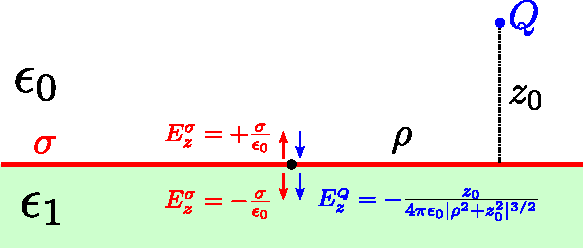
\includegraphics{PointSourceAboveSubstrate.pdf}}
\caption{A point source $Q$ lying a distance $z_0$ above a dielectric
         interface induces a surface charge $\sigma$ on the interface.
         At a distance $\rho$ from the axis of the charge,
         the $z$-directed $\vb E$-field due to $Q$ has the same sign 
         above and below the interface (blue arrows), while that due to
         $\sigma$ changes sign just above and below the interface (red arrows).
        }
\label{PointChargeAboveSlabFigure}
\end{center}
\end{figure}
%####################################################################%

To lend insight into the results of Section \ref{PointOnLayerSection},
I here use simple reasoning to study the position-dependent
surface charge $\sigma(\rho)$
induced on a single dielectric interface (boundary
between two infinite dielectric half-spaces)
by a point charge of strength $Q$ lying on the $z$ axis
at a distance $z_0$ from the interface 
(Figure \ref{PointChargeAboveSlabFigure}).

I assume the source lies above the interface,
so that the $z$-directed field due to the point source
at the interface is negative (points downward).
Including the contribution of the induced surface charge,
the normal electric field just above and below the
dielectric interface at a distance $\rho$ from the origin
reads
%====================================================================%
\numeq{FieldsAboveBelow}
{ E_z(\rho, 0^\pm)
  = 
  \pm\frac{\sigma(\rho)}{2\epsilon_0}
   - \frac{Q z_0}{4\pi \epsilon_0|\rho^2 + z_0^2|^{3/2}}
}
%====================================================================%
The boundary condition is 
%====================================================================%
\begin{align}
\epsilon_0 E_z(\rho,0^+) &= \epsilon_1 E_z(\rho,0^-)
\nonumber
\intertext{or, inserting (\ref{FieldsAboveBelow}),}
\epsilon_0
 \left[
     \frac{\sigma(\rho)}{2\epsilon_0}
   - \frac{Q z_0}{4\pi \epsilon_0|\rho^2 + z_0^2|^{3/2}}
 \right]
&=
\epsilon_1
 \left[
    -\frac{\sigma(\rho)}{2\epsilon_0}
   - \frac{Q z_0}{4\pi \epsilon_0|\rho^2 + z_0^2|^{3/2}}
 \right]
\nonumber
\intertext{whereupon one finds}
\sigma(\rho) &= \pf{\epsilon\subt{0}-\epsilon\subt{1}}
                   {\epsilon\subt{0}+\epsilon\subt{1}}
     \frac{Q z_0}{2\pi |\rho^2 + z_0^2|^{3/2}}.
\label{SigmaRho}
\end{align}
%====================================================================%
The total charge induced on the interface is
%====================================================================%
$$ Q\sups{induced}= 2\pi \int_0^\infty \rho \sigma(\rho) d\rho
   = \pf{\epsilon\subt{0} - \epsilon\subt{1}}
       {\epsilon\subt{0} + \epsilon\subt{1}}Q
$$
%====================================================================%
\textit{independent} of $z_0$.

In the limit $z_0\to 0$, the surface-charge density (\ref{SigmaRho})
tends to a $\delta-$function:
%====================================================================%
$$ \lim_{z\to 0} 
    \sigma(\rho) = \frac{Q\sups{induced}}{2\pi \rho}\delta(\rho).
$$
%====================================================================%
Thus, when the point charge $Q$ lies exactly on the interface,
the sole effect of the interface is to surround $Q$ with
an opposite-sign screening charge, so that the total effective
charge felt is
%====================================================================%
\begin{align*}
 Q\sups{effective} 
&= Q + Q\sups{induced} 
\\
&=\left[ 1 + \pf{\epsilon\subt{0} - \epsilon\subt{1}}
                {\epsilon\subt{0} + \epsilon\subt{1}}
   \right]Q
\\
&=\frac{2\epsilon_0}{\epsilon_0 + \epsilon_1} Q.
\end{align*}
%====================================================================%
This explains why the electrostatics of conductors lying on 
the surface of an infinite dielectric slab in vacuum 
is precisely equivalent to that of conductors in vacuum
with effective permittivity renormalized to 
$$\epsilon_0  \to \frac{1}{1+\frac{\epsilon_1}{\epsilon_0}}.$$

%%%%%%%%%%%%%%%%%%%%%%%%%%%%%%%%%%%%%%%%%%%%%%%%%%%%%%%%%%%%%%%%%%%%%%
%%%%%%%%%%%%%%%%%%%%%%%%%%%%%%%%%%%%%%%%%%%%%%%%%%%%%%%%%%%%%%%%%%%%%%
%%%%%%%%%%%%%%%%%%%%%%%%%%%%%%%%%%%%%%%%%%%%%%%%%%%%%%%%%%%%%%%%%%%%%%
\newpage
\section{Extension to the full-wave case}
\label{FullWaveSection}

\subsection{2D Fourier representation of dyadic Green's functions}

%%%%%%%%%%%%%%%%%%%%%%%%%%%%%%%%%%%%%%%%%%%%%%%%%%%%%%%%%%%%%%%%%%%%%%
\begin{subequations}
\begin{align}
 \vb G(k; \vbrho; z\subt{D}, z\subt{S})
&= \int \frac{d\vb q}{(2\pi)^2}
   \,
   \vb{\wt G}^\pm (k; \vb q)
      e^{i\vb q\cdot \vbrho}
     e^{\pm iq_z(z\subt{D}-z\subt{S})}
\\
 \vb C(k; \vbrho; z\subt{D}, z\subt{S})
&=\int \frac{d\vb q}{(2\pi)^2}
  \, 
  \vb{\wt C}^\pm (k; \vb q) e^{i\vb q\cdot \vbrho}
                   e^{\pm iq_z(z\subt{D}-z\subt{S})}
\end{align}
\label{SpectralGFs}%
\end{subequations}
%%%%%%%%%%%%%%%%%%%%%%%%%%%%%%%%%%%%%%%%%%%%%%%%%%%%%%%%%%%%%%%%%%%%%%
where $\vb q=(q_x,q_y)$ is a two-dimensional Fourier wavevector,
$d\vb q=dq_x dq_y$,
$q_z=\sqrt{k^2-|\vb q|^2}$, $\pm = \text{sign}(z-z^\prime)$,
and
%%%%%%%%%%%%%%%%%%%%%%%%%%%%%%%%%%%%%%%%%%%%%%%%%%%%%%%%%%%%%%%%%%%%%%
\begin{align*}
 \vb{\wt G}^\pm(k; \vb q)
   &=\frac{i}{2 q_z}
     \left[
     \left(\begin{array}{ccc}
      1 & 0 & 0 \\ 
      0 & 1 & 0 \\ 
      0 & 0 & 1
     \end{array}\right)
     -\frac{1}{k^2}
     \left(\begin{array}{ccc}
      q_x^2       & q_x q_y     & \pm q_x q_z \\
      q_yq_x      & q_y^2       & \pm q_y q_z \\
      \pm q_z q_x & \pm q_z q_y & q_z^2
     \end{array}\right)\right]
\\
 \vb{\wt C}^\pm (k; \vb q)
   &=\frac{i}{2q_z k}
     \left(\begin{array}{ccc}
           0 & \pm q_z & -q_y \\
     \mp q_z &       0 &  q_x \\
         q_y &    -q_x &    0
     \end{array}\right).
\end{align*}
%%%%%%%%%%%%%%%%%%%%%%%%%%%%%%%%%%%%%%%%%%%%%%%%%%%%%%%%%%%%%%%%%%%%%%

\begin{align*}
  \vb E &= i k^r Z_0 Z^r \vb G \star \vb K + ik^r \vb C \star \vb N 
\\
  \vb H &= -i k^r        \vb C \star \vb K + \frac{ik^r}{Z_0Z^r} \vb G \star \vb N
\end{align*}

%%%%%%%%%%%%%%%%%%%%%%%%%%%%%%%%%%%%%%%%%%%%%%%%%%%%%%%%%%%%%%%%%%%%%%
\begin{align*}
\wt F_\parallel=
 \left(\begin{array}{c} E_x \\ E_y \\ H_x \\ H_y\end{array}\right)
 &=ik
\end{align*}
%%%%%%%%%%%%%%%%%%%%%%%%%%%%%%%%%%%%%%%%%%%%%%%%%%%%%%%%%%%%%%%%%%%%%%

Tangential fields due to
%%%%%%%%%%%%%%%%%%%%%%%%%%%%%%%%%%%%%%%%%%%%%%%%%%%%%%%%%%%%%%%%%%%%%%
\begin{align*}
\end{align*}
%%%%%%%%%%%%%%%%%%%%%%%%%%%%%%%%%%%%%%%%%%%%%%%%%%%%%%%%%%%%%%%%%%%%%%
\end{document}
